\chapter{Implementation} \label{implementation}
This chapter will elaborate on the test data used as well as the process that was followed to achieve the results in Chapter \ref{results}.
\section{Existing data}
The data used was acquired by \cite{Westhuyzen:2020} for an article assessing the charring rate of both SA-Pine and Eucalyptus.
	For the purpose of this project, only the data obtained from the SA-Pine test was considered and analysed. 
	\subsection{Summary of test}
	The test was conducted on a sample of 100mm by 0.9m x 0.9m panel of cross-laminated SA-pine.
	This sample was then divided into nine cubes of 100 mm x 100 mm x 100 mm.
	%The sample was a 100 mm by 0.9m x 0.9m panel of cross-laminated SA-pine, this sample was then divided into nine cubes of 100 mm x 100 mm x 100 mm.
	Each cube was fitted with seven Type K-thermocouples placed at consecutive 16.5 mm drilled holes, as can be seen in Figure \ref{TC_layout}. 
	The test panel was tested in a furnace and was exposed to the standard ISO 834 Fire curve \ref{firecurve_fig} on one side and room temperature on the other. 
	The panel was exposed to the fire curve for 50 minutes, at which stage near complete de-lamination was observed and the test ended.
	\begin{figure}[H]
	\centering
	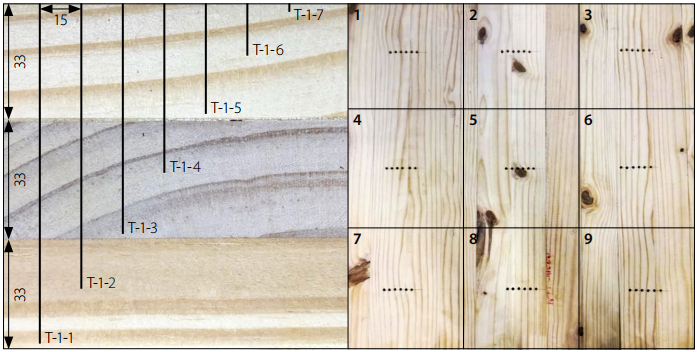
\includegraphics[width=0.75\linewidth]{figures/TC_layout.png}
	\caption{Thermocouple layout in test conducted by \cite{Westhuyzen:2020} cross-section (left) and overall layout (right)}
	\label{TC_layout}
	\end{figure}
	
	\begin{figure}[H]
	\centering 
	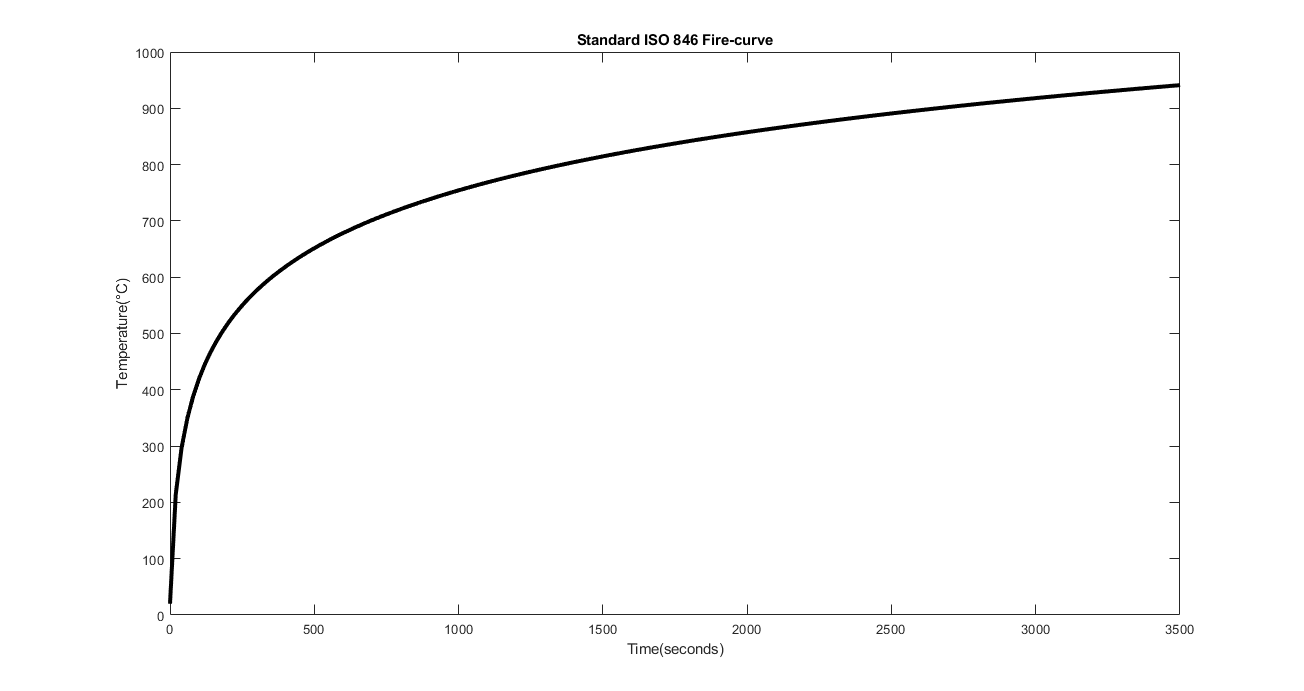
\includegraphics[width=\linewidth]{figures/firecurve.png}
	\caption{Standard ISO fire curve TODO}
	\label{firecurve_fig}
	\end{figure}
	
	\subsection{Potential inaccuracies}
	As with most tests, everything is not always perfect. 
	The potential inaccuracies are discussed below. 
	
	In the data, it was observed that two of the thermocouples broke during testing, this resulted in temperature with a magnitude of $10^{13}$. 
	That temperature is not possible as the highest ever recorded temperature reached was $4\text{x}10^{12}$ and that only occurred in a atomic explosion. %(https://www.insidescience.org/news/hottest-temperature-universe-measured)% 
	This malfunction required that two of the depth measurements were no longer the average between nine samples but instead the average between eight.
	Another inaccuracy that could potentially influence the accuracy of the final result is the accuracy of the depth of the holes in which the thermocouples were placed. 
	%As this was done by hand in the laboratory.
	
	There is also debate about the significance of the contribution of the timber burning to the temperature inside the furnace. 
	For the purposes of this project, it will be assumed that the timber burning does not contribute to the temperature inside the furnace.
	
\section{Finite Element Modelling}
A one-dimensional finite element model that simulates what we expect to obtain from the fire tests based on the simplified K-values provided in EN 1995:1-1-2004 is modified into a function.
This function should provide the temperature of the modelled element based on a specified location and thermal conductivity.
The derivation and adaptation of the model are expanded on below.
	\subsection{Derivation}%"CREATION?"
	%The assumption that the panel is constantly at room temperature on the outside is also inaccurate as there is heat radiating from the panel that increases the temperature surrounding the panel.
	
	\subsection{Existing Model}
	For this project an existing finite element model of heat diffusion by Prof. N de Koker is modified for usage in the Bayes' theorem~\ref{bayes_eq}. 
	This model is used to determine the likelihood function. 
	The current model uses the standard Euro code k-values as well as the specific heat specified in the \citep{Euro:2004}. 
	
	The model discretises the wooden element into 32 different elements. For finite element analysis, there are always more elements used to generate the model than usually evaluated. This is done to improve the accuracy of said model.
	The model is a one dimensional finite element model that takes time differentiation into account.
	
	\subsection{Adapted Model}	
	The model was changed into a function that takes $\kappa$-values and provides a new temperature distribution over the elements for the different $\kappa$-values. 
	This function is used in the posterior calculation to determine the likelihood function.
	


\section{Inversion method}
%here we will discuss everything that we did